\section{Durchführung}
\label{sec:Durchführung}

Der Großteil dieses Versuches wird mit dem Programm XRD-Commander des Diffraktometers durchgeführt.
Zunächst wird dort der maximale Absorber eingeschaltet, damit die Intensität nicht zu hoch ist und Messgeräte eventuell beschädigt werden.
Die Probe wird an die entsprechende Messposition gefahren.
Alle Scan-Ergebnisse dieses Experiments werden in .raw Dateien gespeichert, die in .UXD Dateien umgewandelt werden können damit die Plots für die Auswertung zur Verfügung stehen.

Nun ist es möglich zur Justage drei verschiedene Scans laufen zu lassen, einen Detektorscan, einen Z-Scan und einen Rockingscan.
Alle diese Scans werden mit einer Messdauer pro Position von $\SI{1}{s}$ durchgeführt.

Zuerst wird ein Detektorscan durchgeführt, um den Detektor in die Mitte des Strahls der Röntgenröhre zu fahren.
Die Probe wird in Z-Richtung aus dem Strahl gefahren und die Röhre wird auf $\SI{0}{\degree}$ gestellt.
Der Detektor fährt nun einen kleinen Bereich, etwa $\SI{-0.5}{\degree}$ bis $\SI{0.5}{\degree}$, ab.
Die neue Nulllage des Detektors wird auf das Maximum der aufgenommenen Messung gesetzt.

Die Probe wird wieder in den Strahl gefahren. 
Nun wird die optimale Höhe der Probe bestimmt, diese ist bei halber Abschattung des Strahls erreicht.
Dafür wird ein Z-Scan verwendet. 
Die Probe wird in Z-Richtung verschoben.
Aus den Messdaten wird die Position bei der halben maximalen Intensität entnommen und die Probe wird dorthin gefahren.

Danach folgt ein Rockingscan. 
Dabei wird die Röhre zusammen mit dem Detektor um die Probe gedreht, die Ausrichtung der beiden bleibt dabei gleich, also ist $2\theta = \SI{0}{\degree}$.
Die Funktionsweise dieses Rockingscans ist in \autoref{fig:durch1} dargestellt.
Das Ergebnis sollte ein etwa symmetrisches Dreieick sein, falls das nicht der Fall ist muss in Y-Richtung nachjustiert werden.
Hier werden nun Röhre und Detektor zum Maximum der Verteilung bewegt.

\begin{figure}
    \centering
    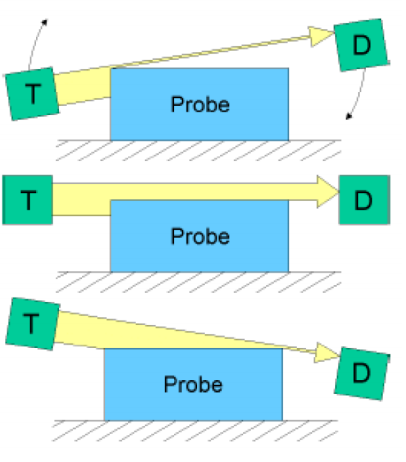
\includegraphics[width=0.4\textwidth]{images/rocking.png}
    \caption{Funktionsweise eines Rockingscans mit $2\theta = \SI{0}{\degree}$. \cite{V44}}
    \label{fig:durch1}
\end{figure}

Die Justierung wird nun noch verfeinert, indem zuerst ein weiterer Z-Scan in einem halb so kleinen Bereich wie zuvor durchgeführt wird.
Dann wird ebenfalls ein weiterer Rockingscan durchgeführt, allerdings stehen sich Röhre und Detektor hier nicht mehr direkt gegenüber, 
sondern es wird $2\theta = \SI{0.3}{\degree}$ eingestellt.
Zuletzt wird wieder ein Z-Scan durchgeführt, bei dem aber Einfalls- und Ausfallswinkel auf $\SI{0.15}{\degree}$ gestellt werden, also wird auch hier $2\theta = \SI{0.3}{\degree}$ eingestellt.
Hier soll wieder die Position der halben Abschattung bestimmt werden, diese ist bei der maximalen Intensität gegeben. 
Das Prinzip dieses Scans ist in \autoref{fig:durch2} gezeigt.

\begin{figure}
    \centering
    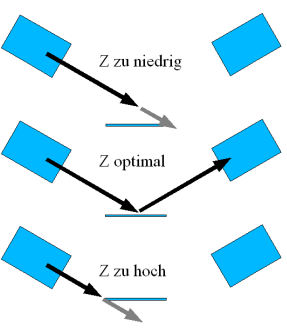
\includegraphics[width=0.4\textwidth]{images/z.png}
    \caption{Funktionsweise eines Z-Scans unter einem Winkel von $2 \theta = \SI{0.30}{\degree}$. \cite{V44}}
    \label{fig:durch2}
\end{figure}

Abschließend findet die eigentliche Messung der Reflektivität der Probe statt.
Der Scantype wird auf Omega/2Theta gestellt und ein Scanbereich von $\SI{0}{\degree}$ bis $\SI{2.5}{\degree}$ eingestellt.
Die Schrittweite soll $\SI{0.005}{\degree}$ betragen bei einer Scanzeit von $\SI{5}{\second}$.
Anschließend wird die Messung erneut durchgeführt, allerdings wird der Detektor um $\SI{0.1}{\degree}$ gegenüber der Röntgenröhre verschoben.
Dies ist der sogenannte diffuse Scan.
